
%%%%%%%%%%%%%%%%%%%%%%%%%%%%%%%%%%%%%%%%%%%%%%%%%%%%%%%%%%%%%%%%%%%%%%%%%%%%%%%%%%%%
% OPL Annex
%
% Recommended 1 page
% The TDP's Robot Description Annex is an appendix of arbitrary length that must be attached at the end of the TDP and summarize the robot's software and hardware technical specifications.
% In this section briefly describe the software and hardware of the robot
%
% Purpose
% It allows the league to track changes in hardware and software trends over time.
% It helps experienced teams to find alternatives to their solutions when looking to improve or conducting benchmarking.
% It serves as a quick reference guide for new teams while preparing their robots.
%%%%%%%%%%%%%%%%%%%%%%%%%%%%%%%%%%%%%%%%%%%%%%%%%%%%%%%%%%%%%%%%%%%%%%%%%%%%%%%%%%%%

\section*{Team Description}
\begin{itemize}[nosep]
  \item \textbf{Team name}: Complubot AZ5
  \item \textbf{Members}:
  \item Juan Casado Ballesteros
  \item Eloy Martín Arconada
  \item Iván Gallego Bravo
  \item \textbf{Address}: Luis Madrona 16 Street, Alcala de Henares, 28804 Madrid, Spain 
  \item \textbf{Phone}: 912801488
  \item \textbf{Email}: az5@complubot.com
  \item \textbf{Webpage}: https://complubot.com/projects/az5
\end{itemize}


%%%%%%%%%%%%%%%%%%%%%%%%%%%%%%%%%%%%%%%%%%%%%%%%%%%%%%%%%%%%%%%%%%%%%%%%%%%%%%%%%%%%
% Parts of the robot
% Devices: bateries, motors, arms, cameras, lidar...
%%%%%%%%%%%%%%%%%%%%%%%%%%%%%%%%%%%%%%%%%%%%%%%%%%%%%%%%%%%%%%%%%%%%%%%%%%%%%%%%%%%%
\section*{Robot's Hardware Description}
\label{sec:annex-OPL}

\begin{itemize}[nosep]
	\item Intel Realsense 2
  \item Slamtec RplidarR A1 
  \item Intel Core i5 8259U @2.30GHzx8, Crucial DDR4 2400 PC4-19200 8GB CL17, Western Digital Blue 3D Nand SATA SSD M.2 2280 250GB
  \item HC-SR05 ultrasonic distance sensor x16
  \item ATtiny 1634 16Mhz x4
  \item ATMega 2560 16 MHz
  \item ATMega 328 16Mhz
  \item VHN2SP30 Motor driver x4
  \item Zippy LiPo battery 3S 11.1V 30C 5800mAh 
  \item Turningy LiPo battery 4S 14.8V 30C 5800mAh 
  \item Highly limit switch ED-62 bumper x8
  \item IG42E-49K Motor winth encoder x4
  \item 152mm Steel Mecanum Wheel with Rubber Rollers (2xLeft, 2xRight)


\end{itemize}

%%%%%%%%%%%%%%%%%%%%%%%%%%%%%%%%%%%%%%%%%%%%%%%%%%%%%%%%%%%%%%%%%%%%%%%%%%%%%%%%%%%%
% Robot SW
% Platform:Operating System
% Navigation
% Recognition
% Speech recognition
% Speech generation
% Arms control...
%%%%%%%%%%%%%%%%%%%%%%%%%%%%%%%%%%%%%%%%%%%%%%%%%%%%%%%%%%%%%%%%%%%%%%%%%%%%%%%%%%%%
\section*{Robot's Software Description}

\begin{itemize}[nosep]
	\item Ubuntu 16.04 LTS with ROS Kinetic
  \item Local navigation and obstacle avoidance Matlab implementation of vector field histogram algorithm
  \item Global navigation Matlab implementation of probabilistic roadmap algorithms for pathplanning and pure pursuit
  \item Mapping lidar based Matlab implementation
  \item Localization ROS implementation of AMCL algorithm
  \item Realsense-ros package for image adquisition and depth perception
  \item Darknet Yolo OpenCV for object and person recognition and hog feature detection for face recognition
\end{itemize}


%%%%%%%%%%%%%%%%%%%%%%%%%%%%%%%%%%%%%%%%%%%%%%%%%%%%%%%%%%%%%%%%%%%%%%%%%%%%%%%%%%%%
% External devices
% 
% Cloud computing
% External computing or actuators
%%%%%%%%%%%%%%%%%%%%%%%%%%%%%%%%%%%%%%%%%%%%%%%%%%%%%%%%%%%%%%%%%%%%%%%%%%%%%%%%%%%%
\section*{External Devices}
\begin{itemize}[nosep]
	\item Ipad Pro used as an onboard interactive screen
\end{itemize}


%%%%%%%%%%%%%%%%%%%%%%%%%%%%%%%%%%%%%%%%%%%%%%%%%%%%%%%%%%%%%%%%%%%%%%%%%%%%%%%%%%%%
% SAS
%
% Geolocalization
% Language processing
%%%%%%%%%%%%%%%%%%%%%%%%%%%%%%%%%%%%%%%%%%%%%%%%%%%%%%%%%%%%%%%%%%%%%%%%%%%%%%%%%%%%
\section*{Cloud Services}
External cloud services are not used.

%%%%%%%%%%%%%%%%%%%%%%%%%%%%%%%%%%%%%%%%%%%%%%%%%%%%%%%%%%%%%%%%%%%%%%%%%%%%%%%%%%%%
% Photo of the robot
%%%%%%%%%%%%%%%%%%%%%%%%%%%%%%%%%%%%%%%%%%%%%%%%%%%%%%%%%%%%%%%%%%%%%%%%%%%%%%%%%%%%
\setlength\intextsep{0pt}
\begin{wrapfigure}[10]{r}{0.3\textwidth}
	\centering
	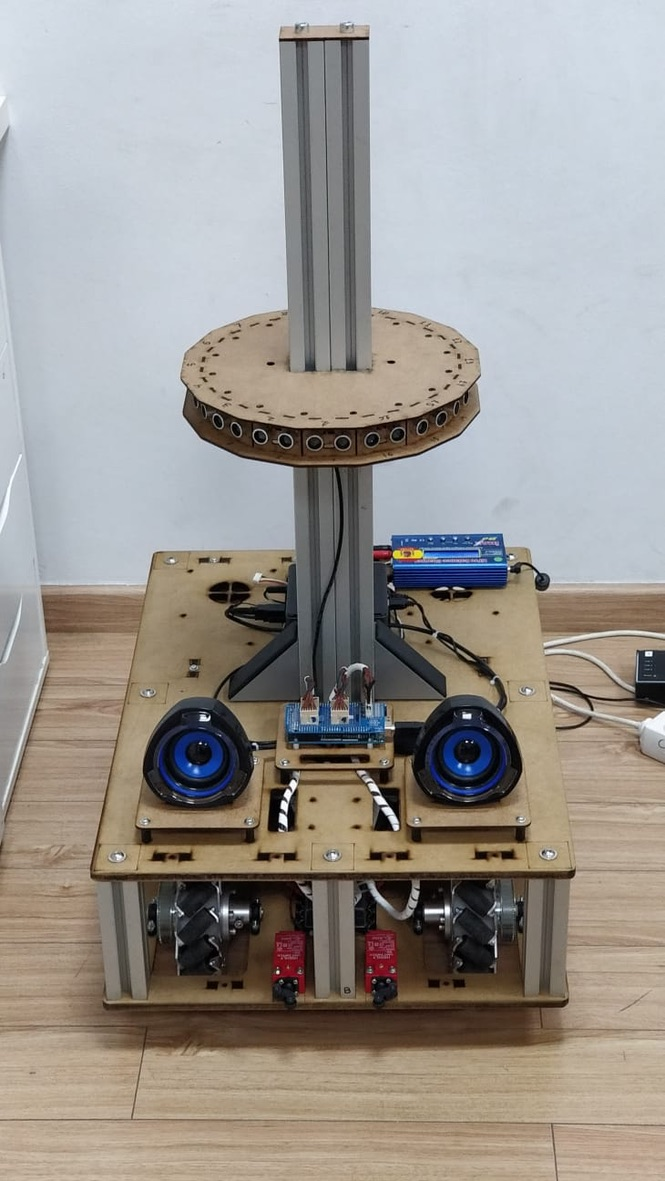
\includegraphics[width=0.4\textwidth]{images/AZ5.jpeg}
	\caption{AZ5}
	\label{fig:wall-e}
\end{wrapfigure}
